% Template for PLoS
% Version 2.0 July 2014
%
% To compile to pdf, run:
% latex plos.template
% bibtex plos.template
% latex plos.template
% latex plos.template
% dvipdf plos.template
%
% % % % % % % % % % % % % % % % % % % % % %
%
% -- IMPORTANT NOTE
%
% Be advised that this is merely a template 
% designed to facilitate accurate translation of manuscript content 
% into our production files. 
%
% This template contains extensive comments intended 
% to minimize problems and delays during our production 
% process. Please follow the template 
% whenever possible.
%
% % % % % % % % % % % % % % % % % % % % % % % 
%
% Once your paper is accepted for publication and enters production, 
% PLEASE REMOVE ALL TRACKED CHANGES in this file and leave only
% the final text of your manuscript.
%
% DO NOT ADD EXTRA PACKAGES TO THIS TEMPLATE unless absolutely necessary.
% Packages included in this template are intentionally
% limited and basic in order to reduce the possibility
% of issues during our production process.
%
% % % % % % % % % % % % % % % % % % % % % % %
%
% -- FIGURES AND TABLES
%
% DO NOT INCLUDE GRAPHICS IN YOUR MANUSCRIPT
% - Figures should be uploaded separately from your manuscript file. 
% - Figures generated using LaTeX should be extracted and removed from the PDF before submission. 
% - Figures containing multiple panels/subfigures must be combined into one image file before submission.
% See http://www.plosone.org/static/figureGuidelines for PLOS figure guidelines.
%
% Tables should be cell-based and may not contain:
% - tabs/spacing/line breaks within cells to alter layout
% - vertically-merged cells (no tabular environments within tabular environments, do not use \multirow)
% - colors, shading, or graphic objects
% See http://www.plosone.org/static/figureGuidelines#tables for table guidelines.
%
% For sideways tables, use the {rotating} package and use \begin{sidewaystable} instead of \begin{table} in the appropriate section. PLOS guidelines do not accomodate sideways figures.
%
% % % % % % % % % % % % % % % % % % % % % % % %
%
% -- EQUATIONS, MATH SYMBOLS, SUBSCRIPTS, AND SUPERSCRIPTS
%
% IMPORTANT
% Below are a few tips to help format your equations and other special characters according to our specifications. For more tips to help reduce the possibility of formatting errors during conversion, please see our LaTeX guidelines at http://www.plosone.org/static/latexGuidelines
%
% Please be sure to include all portions of an equation in the math environment, and for any superscripts or subscripts also include the base number/text. For example, use $mathrm{mm}^2$ instead of mm$^2$ (do not use \textsuperscript command).
%
% DO NOT USE the \rm command to render mathmode characters in roman font, instead use $\mathrm{}$
% For bolding characters in mathmode, please use $\mathbf{}$ 
%
% Please add line breaks to long equations when possible in order to fit our 2-column layout. 
%
% For inline equations, please do not include punctuation within the math environment unless this is part of the equation.
%
% For spaces within the math environment please use the \; or \: commands, even within \text{} (do not use smaller spacing as this does not convert well).
%
%
% % % % % % % % % % % % % % % % % % % % % % % %

\documentclass[10pt]{article}
% amsmath package, useful for mathematical formulas
\usepackage{amsmath}
% amssymb package, useful for mathematical symbols
\usepackage{amssymb}
% cite package, to clean up citations in the main text. Do not remove.
\usepackage{cite}
\usepackage{hyperref}
% line numbers
\usepackage{lineno}
% ligatures disabled
\usepackage{microtype}
\usepackage{todonotes}
\DisableLigatures[f]{encoding = *, family = * }
% rotating package for sideways tables
%\usepackage{rotating}
% If you wish to include algorithms, please use one of the packages below. Also, please see the algorithm section of our LaTeX guidelines (http://www.plosone.org/static/latexGuidelines) for important information about required formatting.
%\usepackage{algorithmic}
%\usepackage{algorithmicx}
% Use doublespacing - comment out for single spacing
%\usepackage{setspace} 
%\doublespacing
% Text layout
\topmargin 0.0cm
\oddsidemargin 0.5cm
\evensidemargin 0.5cm
\textwidth 16cm 
\textheight 21cm
% Bold the 'Figure #' in the caption and separate it with a period
% Captions will be left justified
\usepackage[labelfont=bf,labelsep=period,justification=raggedright]{caption}
% Use the PLoS provided BiBTeX style
\bibliographystyle{plos2009}
% Remove brackets from numbering in List of References
\makeatletter
\renewcommand{\@biblabel}[1]{\quad#1.}
\makeatother

% Our defs 
\def \rr {$R_{t}\ $}

% Leave date blank
\date{}

\pagestyle{myheadings}

%% Include all macros below. Please limit the use of macros.

%% END MACROS SECTION


\begin{document}


% Title must be 150 characters or less
\begin{flushleft}
{\Large
\textbf{Estimating the Attack ratio of Dengue Epidemics without serotype 
information}
}
% Insert Author names, affiliations and corresponding author email.
\\
Flavio Code\c{c}o Coelho$^{1\ast}$, 
Luiz Max de Carvalho$^{2}$, 
\\
\bf{1} Escola de Matem\'atica Aplicada , Funda\c{c}\~ao Getulio Vargas (FGV), 
Rio de Janeiro -- RJ, Brazil.
\\
\bf{2} Programa de Computa\c{c}\~ao Cient\'ifica (PROCC), Funda\c{c}\~ao Oswaldo Cruz, Rio de Janeiro -- RJ, Brazil.
\\
$\ast$ E-mail: fccoelho@fgv.br
\end{flushleft}

% Please keep the abstract between 250 and 300 words
\section*{Abstract}
Our paper is just awesome.
% Please keep the Author Summary between 150 and 200 words
% Use first person. PLOS ONE authors please skip this step. 
% Author Summary not valid for PLOS ONE submissions.   
\section*{Author Summary}

\section*{Introduction}

Dengue is a disease which is caused by 4 different types of viruses 
which co-circulate between the vector and human populations. immunity is 
considered permanent after the exposure of humans to each of the viruses but 
cross immunity is considered very limited[ref].
Thus, the proportions of viral types co-circulating at any point in time is 
strongly dependent on previous incidence of the disease, which determines the 
number of susceptibles for each viral type at any point in time.

Dengue transmission is conditioned on temperature, due to its effects on the 
vector reproduction.
In places with sufficient temperature variations dengue is a summer disease 
mainly. 

Determining the viral types in circulation during an epidemic is 
expensive, as it requires virus isolation and reverse-transcriptase-PCR. 
Therefore only a very limited number of samples are examined on any epidemic. 
Besides, mild cases are rarely detected let alone tested for dengue.

Dengue in Brazil is a disease which is well in its way to 
endemicity but not yet stable, therefore co-circulation patterns have not yet 
reached a steady state as has been demonstrated for certain countries in 
south-east asia which have had the disease much longer.

In the particular case of Dengue fever in Brazil, with four circulating 
serotypes, it can be very challenging to parameterize a simulation starting at 
any time other than when the date the disease was reintroduced in the country 
in the late 1980s and even so, without virological survey data from time to 
time, to inform on the mixing of viruses in circulation, it is virtually 
impossible to predict, by simulation alone, the imunological state of the 
population at any point in the future.

For SIR-like models, the relevant initial values are the number of infectious 
and susceptible  individuals. 
The number of infectious individuals are less challenging to determine, because 
the get very small during the winters and can be derived from incidence data  
with is monitored continuously.
The real challenge is to determine the number of susceptibles to 
a particular strain right at the beginning of the dengue season.

Multiple factors contribute to the dificulty in estimating the number of 
susceptibles in the population, first and foremost is the fact that dengue
confers permanent immunity within serotypes but with only short-lived 
cross-immunity. 
Secondly, there are a larger number of asymptomatic cases in 
any epidemic, which nevertheless acquire immunity. It is estimated that for 
every case reported, 10-20 are not seen by health authorities (personnal 
communication).
Thirdly, under-reporting is a serious issue in Brazil. 
Duarte and Fran\c{c}a\cite{duarte_data_2006}, estimated 
the sensitivity of dengue reporting for hospitalized patients in 
Belo-Horizonte, Brazil to be of 63\%, 
meaning that aproximately 37\% of the suspected dengue cases go unreported.  
Lastly, demography and migrations affect the number of susceptible in ways which 
are not easy to determine.

The initial number of susceptibles -- $S_0$ -- is a a very powerful parameter 
with regards to epidemic risk.
Its value affects directly the local $R_0$, thus being intrumental in predicting 
epidemics, but it also affects the speed and size of the epidemic.

In this paper, we estimate the number of susceptibles, allowing for 
discontinuities right before every epidemic in the last 18 years. 
Through this method we hope to detect drastic changes in the mixture of 
susceptibles cause by the replacement of the predominant serotype, which 
can redefine susceptibility for the following season.

To accomplish this we use a simplified model of 
dengue transmission based on a Susceptible-infecctious-Removed (SIR) model. 
Since Dengue is not caused by a single pathogen, but by four separate strains 
with limited cross-immunity, when we talk about number of susceptibles, in the 
context of a single serotype SIR model, we are actually referring to the sum of 
the susceptibles to the currently circulating serotypes at any given time. 

Some information is available about the predominant serotypes during the 
period of study\cite{macedo_virological_2013}. 

The estimation of the  number of susceptibles have been attempted 
before, for other diseases\cite{bjornstad_dynamics_2002, 
wallinga_reconstruction_2003}. These methods try to reconstruct the entire 
series of infectious and susceptibles for measles 
outbreaks from case data.\todo[inline]{anyone else?} In the case of Dengue the 
series of susceptibles to all possible serotypes, cannot be reconstructed based 
solely on a deterministic transmission model, since the arrival/re-emergenge of 
new serotypes (which are a stochastic events) can change drastically the pool 
of susceptibles throwing off any sequential estimation of the dynamics. 
Adopting a multi-strain transmission model, does not help because of 
insufficient information about the proportions of each serotype in case data.

The authors have applied similar methods as used here, to estimate the number 
of susceptibles for the predominant strain of influenza at the beginning of  
influenza seasons in europe\cite{pone2011}.


\section*{Methods}

\subsection*{Estimating the reproductive number}

In monitoring of infectious diseases, it is important to assess whether the 
incidence of a a particular disease is increasing significantly, in order to 
decide to take preventive measures.
The effective reproductive number at time $t$, \rr, can be understood as a 
real-time estimate of the basic reproductive number ($R_{0}$) and is defined as 
the average number of secondary cases per primary case at time $t$.
Here we derive confidence/credibility bounds for the uncertainty about the 
estimate of the effective reproductive number $R_t$ under the assumption that 
reported disease counts are Poisson distributed.
It is shown that one can construct a conservative confidence interval for \rr 
using the induced probability distribution that results from the approach of 
\cite{mantel}.

Let $Y_t$ be the number of reported disease cases for a particular time $t \in 
(0, T)$.
\cite{nishiura} extend the theory developed by \cite{stallybrass} and propose 
to estimate \rr as
\begin{equation}
\label{eq:Rtestimate}
R_t = \left( \frac{Y_{t+1}}{Y_t}\right)^{1/n}
\end{equation}
where $n$ is taken to be the ratio between the length of reporting interval and 
the mean generation time of the disease.
Here we are interested in the simpler case $n=1$.
If \rr is to be used as a decision tool, one needs to be able to quantify the 
uncertainty about estimate in equation~\ref{eq:Rtestimate}. 
Here we detail how to obtain confidence intervals for \rr, exploring two 
approaches under the assumption that the counts $Y_t$ are Poisson distributed 
for all $t$.

First we explore the approach of \cite{mantel}, whose objective is to obtain 
confidence intervals for the ratio of two Poisson counts. 
Let $Y_{t} \sim Poisson(\lambda_t)$ and $Y_{t+1} \sim Poisson(\lambda_{t+1})$ 
and define $S = Y_{t} + Y_{t+1}$.
The authors then proceed to note that by conditioning on the sum $S$
\begin{align}
\label{eq:binlike}
Y_{t+1} | S &\sim Binomial(S, \theta_t) \\
\theta_t &= \frac{\lambda_{t+1}}{\lambda_{t} + \lambda_{t+1}}
\end{align}
Let $c_{\alpha}(\theta_t) = \{\theta_t^{(L)} , \theta_t^{(U)} \}$ be such that 
$Pr(\theta_t^{(L)}<\theta_t <\theta_t^{(U)}) = \alpha$.
Analogously, define $c_{\alpha}(R_t) = \{R_t^{(L)} , R_t^{(U)} \}$ such that 
$Pr(R_t^{(L)}<R_t<R_t^{(U)}) = \alpha$.
\cite{mantel} show that one can construct a $100\alpha \%$ confidence interval 
for \rr by noting that
\begin{align}
 R_t^{(L)} &= \frac{\theta_t^{(L)}}{(1-\theta_t^{(L)})}\\
 R_t^{(U)} &= \frac{\theta_t^{(U)}}{(1-\theta_t^{(U)})}
\end{align}

Many authors have derived $c_{\alpha}(\theta_t)$ following orthodox approaches 
such as those of \cite{wilson} and \cite{clopper}, mainly for simplicity 
reasons.
We choose instead to take a Bayesian approach and use the  $100\alpha \%$ 
posterior credibility interval for $\theta_t$ as $c_{\alpha}(\theta_t)$.
If we choose the conjugate beta prior with parameters $a_0$ and $b_0$ for the 
binomial likelihood in (\ref{eq:binlike}), the posterior distribution for 
$\theta_t$ is
\begin{equation}
\label{eq:thetapost}
p(\theta_t| Y_{t+1}, S) \sim Beta(Y_{t+1} + a_0, Y_t + b_0)
\end{equation}
Equation~(\ref{eq:thetapost}) tells us that the induced distribution of $R_t$ is 
a beta prime with parameters $ a_1 = Y_{t+1} + a_0$ and $b_1 =  Y_t + b_0$.
The density of this induced distribution  $f_P(R_t)$ is then 
\begin{equation}
\label{eq:densityMantel}
f_P(R_t| a_1, b_1) = \frac{\Gamma(a_1 + b_1)}{\Gamma(a_1)\Gamma(b_1)} R_t^{a_1 - 
1} (1 + R_t)^{-(a_1 + b_1)}
\end{equation}
Thus, the expectation of \rr under $f_P$ is $a_1/(b_1 - 1)$ and its variance is 
$a_1(a_1 + b_1 - 1)/\left((b_1 - 2)(b_1 - 1)^2 \right) $.

Since when $R_t > 1$ indicates sustained transmission, one may be interested in 
computing the probability of this event.
By noting that
\begin{align}
\label{cumprobMantel}
Pr(R_t > 1) &= 1 - \int_0^1 f_P(r)dr \\
            &= 1- Pr(\theta_t < \frac{1}{2})
\end{align}
one can avoid dealing with the density in~(\ref{eq:densityMantel}) directly.

The data used to fit the model consists of weekly incidence from 1996 to 2014 
in the city of Rio de Janeiro, Brazil.

\subsection*{The model}

A Susceptible-Infectious-Removed (SIR) model is proposed to model dengue dynamics.
In the traditional formulation of the model, transmission is governed by a 
transmission rate $\beta$ and recovery happens at a rate $\tau$.

As the epidemic progresses, the effective transmission  rate changes and is
\begin{equation} 
 \label{eq:effbeta}
 \beta(t) = \frac{R_t\cdot\tau}{S_0}
\end{equation}
where $R_t$ is the effective reproductive number as defined 
in~\ref{eq:Rtestimate}.
We parameterize our model with the varying transmission using the system of 
ordinary differential equations
\begin{align}
 \frac{dS}{dt} &= -\beta(t)SI \\
 \frac{dI}{dt} &= \beta(t)SI - \tau I&\\
 \frac{dR}{dt} &= \tau I&
\end{align}
where $S + I + R = 1 \: \forall\: t$. % \in [T_0, T_1]$. 
This is a rather simplified model, in which, for instance, the vector is left 
out.
Also, although there probably are multiple circulating serotypes, our approach
does not discriminate between them due to the lack of serotype-specific data.


\subsection*{Bayesian parameter estimation}

For the fitting procedure the time series was divided into $J=10$ epidemic 
windows that corresponded to significant raises in incidence and normalized to 
lie on the $[0,1]$ interval.
Also, as the numerical integration routine needs to treat $\beta(t)$ as a
continuous function of time because of the variable step size, we used linear 
interpolation to obtain values of $R_t$ for any time point.

We take a Bayesian approach to the estimation of $S_0$ for each window.
For a given interval $j = \{ t_j^{\text{start}}, t_j^{\text{end}} \} $ we 
observe an incidence time series $\mathbf{Y_{j}}$.
We are thus interested in the posterior distribution
\begin{equation}
 \label{eq:S0post}
 p(S_{0j}|\mathbf{Y_{j}}) \propto l(\mathbf{Y_{j}}|S_{0j}, R_t, m,  \tau 
)\pi(S_{0j}) 
\end{equation}
The likelihood $l(\mathbf{Y_{j}}|\cdot)$ is assumed to be a Normal distribution 
with fixed variance $\sigma^2$.
In this estimation procedure we kept $R_t$ fixed at fixed at the posterior mean 
obtained as described in TextS1 and fixed $\tau = 1/7\: \text{days}^{-1}$.
% \subsubsection*{Priors}
To complete the inference, we need to specify prior distributions for the 
parameters of interest.
We place a flat $\text{Beta}(1, 1)$ prior on $S_{0j}\:\forall j$
% 
% \begin{align}
%  S_{0j} &\sim Beta(1, 1) \\
%        m &\sim \\
% \end{align}


% \subsubsection*{Posterior approximation}

To approximate the posterior in~(\ref{eq:S0post}) we use Markov chain Monte 
Carlo techiniques implemented in the Bayesian inference with Python 
(BIP)~\cite{pone2011} available at 
\url{http://code.google.com/p/bayesian-inference/}.
BIP uses a Differential Evolution Adaptive Metropolis (DREAM)~\cite{vrugt2008} 
scheme that efficiently samples from high-dimensional joint distributions using 
multiple adaptive chains running in parallel with delayed rejection.
In this study we used one chain per parameter, i.e, 3 chains for each run.
The chains were run until $5000$ samples were obtained after discarding $500$ 
burn-in samples.
Convergence of the parallel chains was verified at every 100 iterations by the 
calculation of the Gelman-Rubins' R convergence diagnostic~\cite{brooks1998}.

% Results and Discussion can be combined.
\section*{Results}
% We only support three levels of headings, please do not create a heading level below \subsubsection.
%\subsection*{Subsection 1}
\section*{Discussion}
% Do NOT remove this, even if you are not including acknowledgments.
\section*{Acknowledgments}
LMC is grateful to Dr. Leonardo Bastos for useful discussions on the 
posterior inference for $R(t)$.

\bibliography{lm1}
\section*{Figure Legends}
% This section is for figure legends only, do not include
% graphics in your manuscript file.
%
%\begin{figure}
%\caption{
%{\bf Bold the first sentence.}  Rest of figure caption.  
%}
%\label{Figure_label}
%\end{figure}
\begin{figure}
\begin{center}
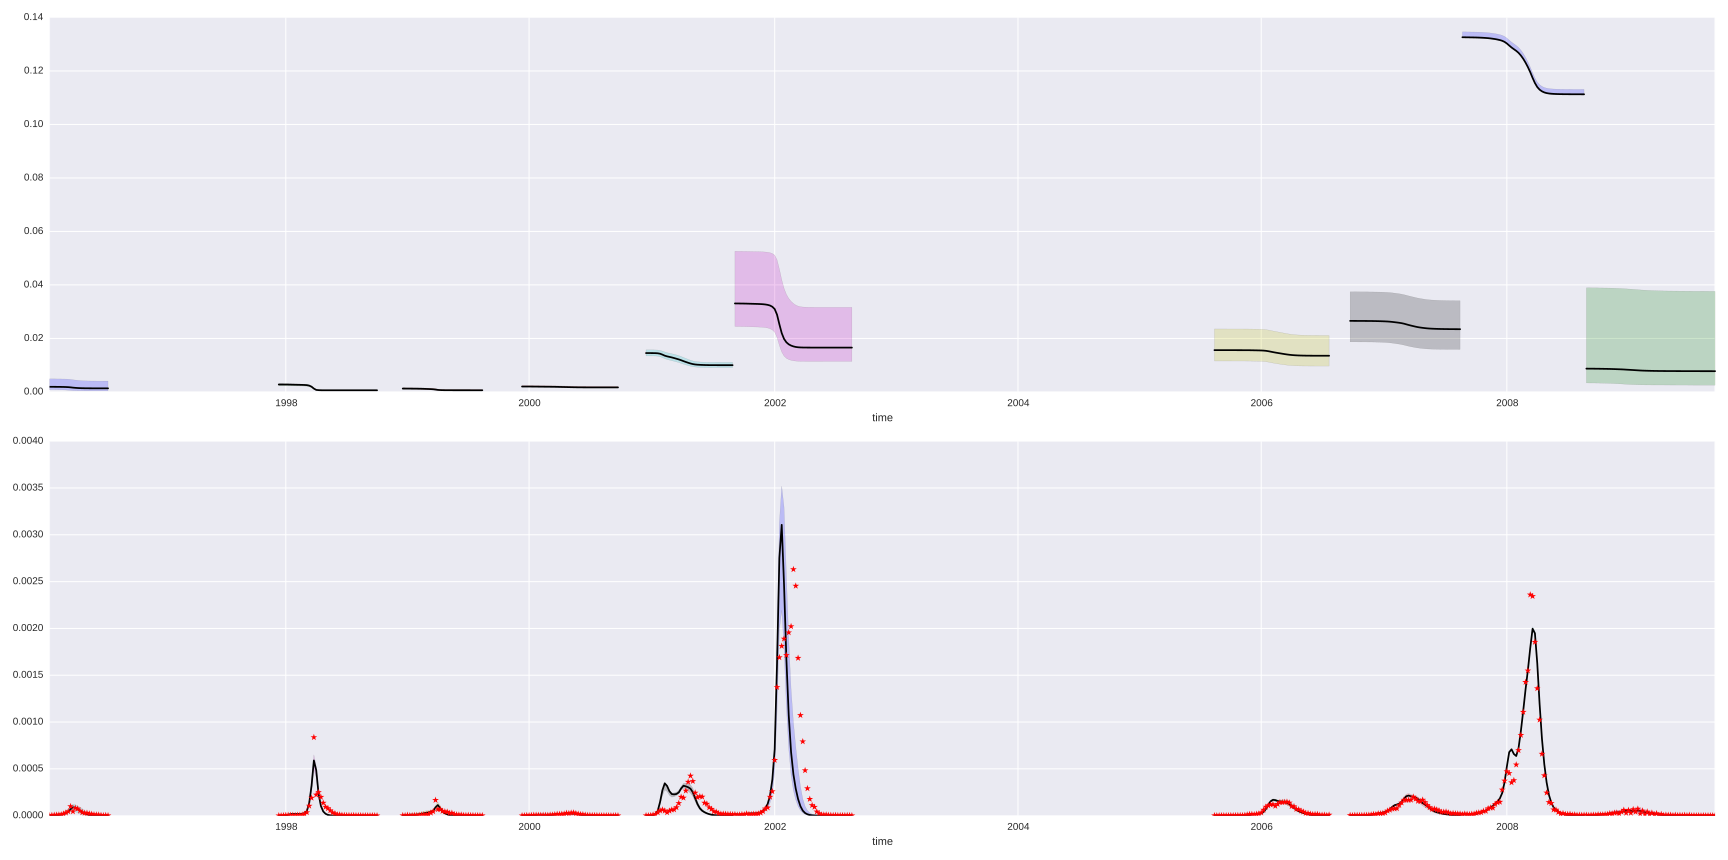
\includegraphics[width=.9\textwidth]{./plots/concat_SI.png}
\end{center}
\caption{
{\bf Bold the first sentence.}  Rest of figure caption.  
}
\label{Fig:S0}
\end{figure}



\section*{Tables}
% 
% See introductory notes if you wish to include sideways tables.
%
% NOTE: Please look over our table guidelines at http://www.plosone.org/static/figureGuidelines#tables to make sure that your tables meet our requirements. Certain types of spacing, cell merging, and other formatting tricks may have unintended results and will be returned for revision.
%
%\begin{table}[!ht]
%\caption{
%\bf{Table title}}
%\begin{tabular}{|c|c|c|}
%table information
%\end{tabular}
%\begin{flushleft}Table caption
%\end{flushleft}
%\label{tab:label}
% \end{table}

\section*{Supporting Information Legends}
%
% Please enter your Supporting Information captions below in the following format:
%\item{\bf Figure SX. Enter mandatory title here.} Enter optional descriptive information here.
% 
%\begin{description}
%\item {\bf}
%\item {\bf}
%\end{description}

\end{document}

